\section{Digital Design For ASICS}
Moderne FPGA-Designs haben viel gemeinsam mit modernen ASIC-Designs. Trotzdem gibt es einige grundlegende Unterschiede.
\subsection{Zielanwendungen}
Im Vergleich zu FPGA-Designs sprechen die ASIC-Designs einen anderen Markt an. ASIC-Designs eignen sich in der Regel für Anwendungen mit hohem Produktionsvolumen, d.h. mindestens 100'000 Stücke pro Jahr, weil die NRE Kosten (einmalige Entwicklungskosten) sehr hoch sind. 
\paragraph{Gesamtkosten pro Einheit} 
$c=\frac{c_0}{n}+c_1$ \ \ \ c\textsubscript{0}: Summe der einmaligen Entwicklungskosten $\rightarrow$ konstant // n: Anzahl der entwickelten ASICS // c\textsubscript{1}: Kosteninkrement pro erzeugter Schaltung (für Rohwafer, Waferbearbeitung, Prüfung, Verpackung, Logistik usw.) $\rightarrow$ linear steigend
\begin{multicols}{2}
\textbf{c\textsubscript{0} ist ist abhängig von:} 
\begin{compactitem}
    \item Herstellungsprozess und Prozessoptionen, die die Masken- und die Waferherstellungskosten bestimmen
    \item Lizenzkosten und Lizenzgebühren für IP-Cores
    \item CAD-Tool-Kosten
    \item Engineering-Kosten für Design der Schaltung und Design der Testlösung
    \item Aufbau der Versorgungs- und Logistikkette
    \item etc.
\end{compactitem}
\textbf{c\textsubscript{1} ist abhängig von:} 
\begin{compactitem}
    \item Schaltungsgrösse
    \item Testzeit
    \item Herstellungsertrag
    \item Verpackungskosten
    \item etc.
\end{compactitem}
\ \\ \ \\
\end{multicols}
Beim FPGA-Design ist c\textsubscript{0} relativ klein im Vergleich zum ASIC-Design. Die Startkosten bei c\textsubscript{1} sind beim FPGA-Design tiefer als im ASIC-Design. Jedoch steigen die Kosten beim FPGA-Design steiler an als beim ASIC-Design. Der Schnittpunkt der beiden Gesamtkosten ergibt ungefähr Volumengrenze zwischen FPGA- und ASIC-Entwicklung. 
\subsection{Design Flow}
\begin{figure}[H]
    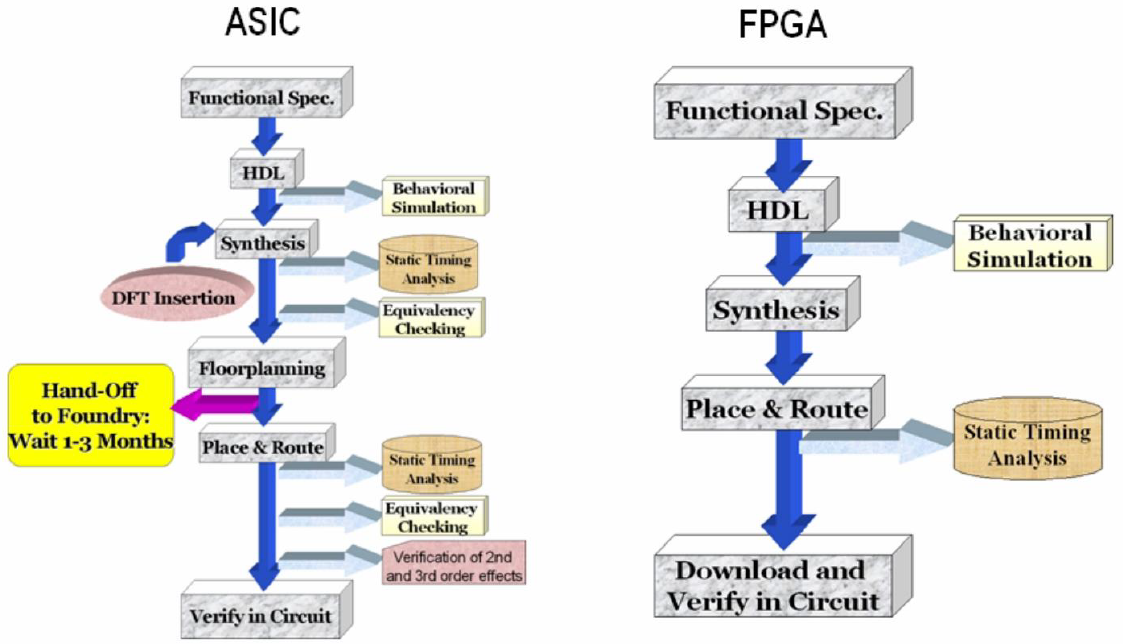
\includegraphics[width=1\textwidth]{images/ASIC_FPGA.png}
\end{figure}
\subsubsection{Synthese (FPGA vs. ASIC)}
\paragraph{FPGA}
\begin{compactitem}
    \item Target device bestimmen/auswählen (Hersteller, Familie, FPGA Typ)
    \item Wahl des Sythetisiertools
    \item Constraints hinzufügen (im XDC-Format) 
    \item Für kombinatorischen Teil werden LUTs und für den sequentiellen Teil FF erzeugt. 
    \item Hat Scankette eingebaut, da Scan und JTAG beim Programmieren gebraucht wird.
\end{compactitem}
\paragraph{ASIC}
\begin{compactitem}
    \item Wahl des Designhouse: ASIC-Design erfordert Wissen, Erfahrung und Infrastruktur, welche nicht immer vorhanden ist $\rightarrow$ evtl. Designhouse
    \item Wahl des Sythetisiertools (teuer!)
    \item Wahl der Technologie
    \item Wahl der digitalen Zellenbibliothek
    \begin{compactitem}
        \item High Density (9 or 10 tracks high): Mittlere Transistorgrösse für hohe Dichte und gute Performance, low power
        \item Ultra-High Density (7 or 8 tracks high): Kleine Transistorgrösse für sehr hohe Dichte und low power
        \item High Performance (12 tracks high): Grosse Transistorgrösse für optimale Geschwindigkeit, auch low power features
    \end{compactitem}
    \item Wahl der Soft- und Hard IP Blöcke (Block RAMs, DSP Blöcke, etc. sind normalerweise nicht vorhanden $\rightarrow$ kaufen
    \item Constraints hinzufügen (im SDC-Format) 
    \item Erzeugung generische Netzliste (im .edif Format), welche grundlegende boolesche Funktionen, die keine realen Gatter mit Layout und Timing sind, verwendet. Technologieunabhängig.
    \item Mapping, bei welchem die Grundfunktionen auf reale Zellen aus der Zellbibliothek abgebildet werden.
    \item Hat keine eingebauten Testfunktionen. Die Testlogik wird erzeugt und während der Synthese hinzugefügt $\rightarrow$ FFs werden durch Scan-FFs ersetzt. Scan-Kette wird erzeugt.
\end{compactitem}

\subsubsection{Floorplanning}
Floorplanning bezieht sich darauf, einzelne Elemente, Schaltungsblöcke und IOs vorläufig auf einem physikalischen Layout zu platzieren. Im FPGA-Design ist das Floorplanning ein Teil des Place and Route (Hinzufügen von Physical Constraints).

\subsubsection{Place and Route (FPGA vs. ASIC)}
\paragraph{FPGA}
\begin{compactitem}
        \item Zuweisung der verschiedenen Netzlistenelemente zu vorhandenen LUTs, FFs und Hardware-Makros auf dem FPGA-Chip $\rightarrow$ wird automatisch bei ''Run Implementation'' und ''Generating Bitstream'' zugewiesen. 
        \item Einfluss nur bedingt via Physical Constraints
\end{compactitem}
\paragraph{ASIC}
Besitzt mehrere Teilschritte:
\begin{compactitem}
        \item Power Planning: Generiert den Powerring, der VDD und VSS um den gesamten Chip erzeugt. Für horizontale Verbindungen und vertikale Verbindungen werden unterschiedliche Metallschichten verwendet.
        \item Definition Power Grid für Standardzellen: Abhängig von der ausgewählten Standardzellenbibliothek und ihrer charakteristischen Höhe wird das Gitter für VDD und VSS der Standardzellen erzeugt.
        \item Platzierung der Standardzellen (iterativer Prozess): Standardzellen werden mit einem bestimmten Dichtefaktor platziert, was bedeutet, dass ein gewisser Raum zwischen den Zellen frei bleibt. Dann versucht das Tool, die Leitungen zwischen den Zellen zu setzen. Wenn das Routing nicht erfolgreich war, startet der Prozess erneut mit einem neuen Placement. Wenn das Routing erfolgreich war, kann es weiterhin sinnvoll sein, den Prozess fortzusetzen, indem versucht wird, die Dichte zu erhöhen und dadurch die Gesamtgrösse des Chips zu verringern.
        \item Erzeugung der Clockstruktur: Alle sequentiellen Zellen müssen mit einem Taktsignal verbunden sein. Dieses Signal muss bestimmten Qualitätsanforderungen entsprechen. Das Ergebnis der Taktgenerierung ist ein Taktnetzwerk, das aus Puffern besteht, die in Form eines Baumes mit Puffern verschiedener Treiberstärken verbunden sind, so dass der Clock Skew an den einzelnen Endpunkten minimiert wird.
        \item Nach erfolgreichem Place and Routing wird der Leerraum in den Standardzellenfeldern mit sogenannten Füllerzellen gefüllt, um "Löcher" in den Zeilen zu schliessen. Dies ist notwendig, um kontinuierliche p- und n-Wannen entlang einer ganzen Standardzellenreihe zu haben.
\end{compactitem}
\subsubsection{Verifikation FPGA vs. ASIC}
\paragraph{FPGA}
Verifikation gleich nach herunterladen der Programmdaten möglich. Man muss nicht auf einen Prototypen warten.
\paragraph{ASIC}
Verifikation nicht gleich möglich. Folgende Schritte müssen VOR der Verifikation vollzogen werden: 
\begin{compactitem}
        \item Sign-off: Daten der Prdouktion übermitteln und prüfen lassen
        \item Generierung der Maske 
        \item Waferbearbeitung
        \item Wafertests, Wafer Dicing (schneiden), Verpacken
\end{compactitem}
